\newpage
\section{Auswertung}
\label{sec:Auswertung}

\subsection{Messung der Magnetfelder verschiedener Spulen}

In den folgenden Untersabschnitten sind die Ergbinsse der verschiedenen Messungen der magnetischen
Flussdichte dargestellt. 

\subsubsection{Lange Spule}

  \begin{table}
    \centering
    \caption{Messdaten der langen Spule.}
    \label{tab:lang}
    \sisetup{table-format=1.3}
    \begin{tabular}{S[table-format=2] S}
    \toprule
    {$x \:/\: \si{\cm}$} & {$B \:/\: \si{\milli\tesla}$}\\
    \midrule
          4 & 0.079\\
          3 & 0.139\\
          2 & 0.258\\
          1 & 0.506\\
          0 & 0.971\\
          -1 & 1.524\\
          -2 & 1.888\\
          -3 & 2.077\\
          -4 & 2.165\\
          -5 & 2.213\\
        \bottomrule
      \end{tabular}
    \end{table}

\begin{figure}
  \centering
  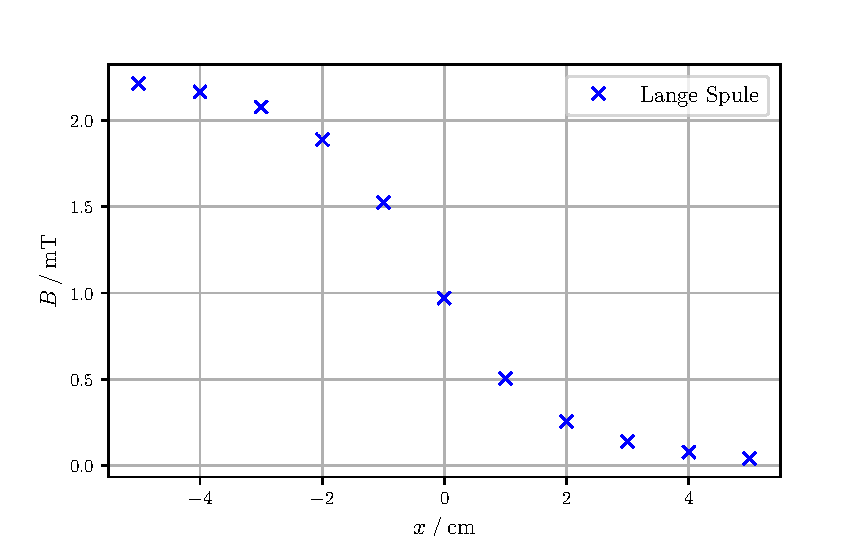
\includegraphics[width=\textwidth]{build/lange_Spule.pdf}
  \caption{Messdaten der langen Spule.}\label{fig:lang}
\end{figure}

\newpage

\subsubsection{Kurze Spule}
  \begin{table}
    \centering
    \caption{Messdaten der kurzen Spule.}
    \label{tab:kurz}
    \sisetup{table-format=1.3}
    \begin{tabular}{S[table-format=2] S}
    \toprule
    {$x \:/\: \si{\cm}$} & {$B \:/\: \si{\milli\tesla}$}\\
    \midrule
          5 & 0.048\\
          4 & 0.076\\
          3 & 0.131\\
          2 & 0.247\\
          1 & 0.470\\
          0 & 0.886\\
          -1 & 1.405\\
          -2 & 1.770\\
          -3 & 1.882\\
          -4 & 1.812\\
          -5 & 1.530\\
          \bottomrule
  \end{tabular}
\end{table}

\begin{figure}
  \centering
  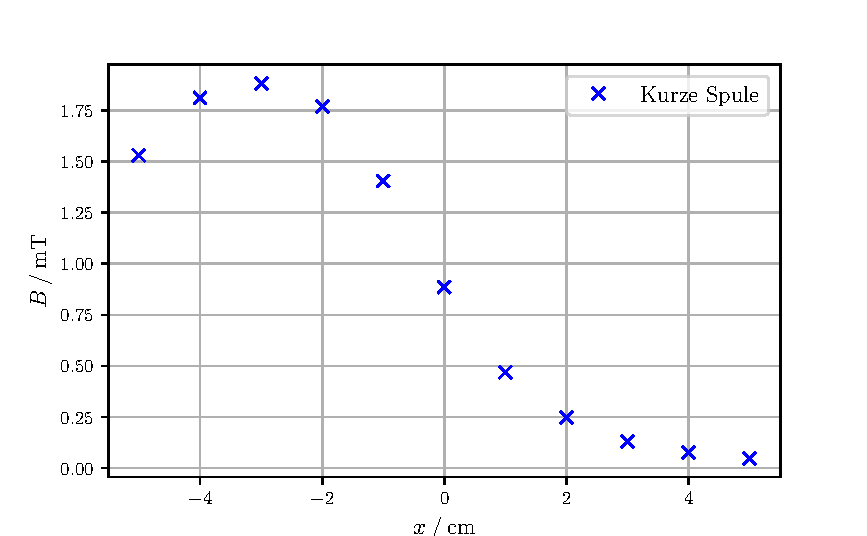
\includegraphics[width=\textwidth]{build/kurze_Spule.pdf}
  \caption{Messdaten der kurzen Spule.}\label{fig:kurz}
\end{figure}

\newpage
\subsubsection{Dicke Spule}
  \begin{table}
    \centering
    \caption{Messdaten der dicken Spule.}
    \label{tab:dick}
    \sisetup{table-format=1.3}
    \begin{tabular}{S[table-format=2] S}
    \toprule
    {$x \:/\: \si{\cm}$} & {$B \:/\: \si{\milli\tesla}$}\\
    \midrule
        5 & 1.56\\
        4 & 2.00\\
        3 & 2.58\\
        2 & 3.31\\
        1 & 4.22\\
        0 & 5.18\\
        -1 & 6.13\\
        -2 & 7.01\\
        -3 & 7.64\\
        -4 & 7.99\\
        -5 & 8.03\\
        \bottomrule
      \end{tabular}
    \end{table}


\begin{figure}
  \centering
  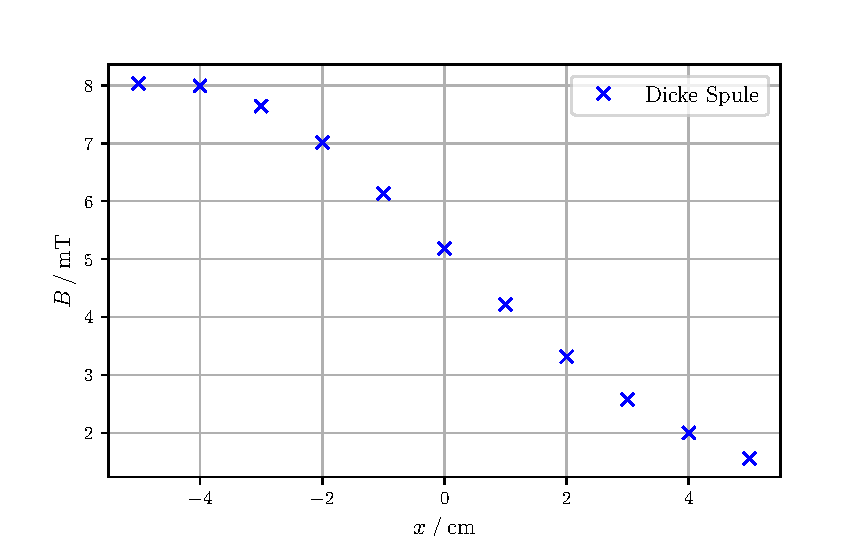
\includegraphics[width=\textwidth]{build/dicke_Spule.pdf}
  \caption{Messdaten der dicken Spule.}\label{fig:dick}
\end{figure}

\newpage
\subsection{Helmholtz-Spulen-Paar}

Die Messdaten bezüglich der Helmholtz-Spulen können der Tabelle \ref{tab:helmholtz}
entnommen werden. In den einzelnen Abbildungen (\ref{fig:H12}; \ref{fig:H6}; \ref{fig:H18}) 
ist der magnetische Fluss jeweils bei verschiedenen Spulenabständen in Abhängigkeit der Stromstärke aufgetragen.
Man kann im vergrößerten Plot (\ref{fig:H6_1}) die Homogenität des B-Feldes zwischen den beiden Spulen erkennen.
Dies entspricht den Erwartungen der Messung, da dort die beiden Spulen die eigentlichen Eigenschaften
einer tatsächlichen Helmholtz-Spule erfüllen.(Siehe \ref{sec:Theorie})


  \begin{table}
    \centering
    \caption{Messdaten des Helmholtz-Spulen-Paares.}
    \label{tab:helmholtz}
    \begin{tabular}{S[table-format=2.1] S[table-format=1.2] S[table-format=2.1] S[table-format=1.3] S[table-format=2.1] S[table-format=1.3]}
    \toprule
    \multicolumn{2}{l}{Spulenabstand: $12.5 \si{\cm}$} & \multicolumn{2}{l}{Spulenabstand: $6.25 \si{\cm}$} & \multicolumn{2}{l}{Spulenabstand: $18.75 \si{\cm}$}\\
      \cmidrule(lr){1-2}\cmidrule(lr){3-4} \cmidrule(lr){5-6}
    {$x \:/\: \si{\cm}$} & {$B \:/\: \si{\milli\tesla}$} & {$x \:/\: \si{\cm}$} & {$B \:/\: \si{\milli\tesla}$} & {$x \:/\: \si{\cm}$} & {$B \:/\: \si{\milli\tesla}$}\\
    \midrule
       3.0 & 4.34 & 2.2 & 6.917 & 3.0 & 3.683\\
       4.0 & 4.02 & 2.3 & 6.919 & 4.0 & 3.245\\
       5.0 & 3.78 & 2.4 & 6.924 & 5.0 & 2.780\\
       6.0 & 3.70 & 2.5 & 6.921 & 6.0 & 2.406\\
       7.0 & 3.76 & 2.6 & 6.925 & 7.0 & 2.129\\
       8.0 & 3.96 & 2.7 & 6.924 & 8.0 & 1.960\\
       9.0 & 4.29 & 9.0 & 4.546 & 9.0 & 1.888\\
       15.0 & 4.08 & 10.0 & 3.804 & 10.0 & 1.927\\
       16.0 & 3.50 & 11.0 & 3.126 & 11.0 & 2.057\\
       17.0 & 2.91 & 13.0 & 2.048 & 12.0 & 2.298\\
       18.0 & 2.37 & 15.0 & 1.372 & 13.0 & 2.636\\
       19.0 & 1.94 & 17.0 & 0.947 & 14.0 & 3.042\\
       20.0 & 1.54 & 19.0 & 0.684 & 22.0 & 3.473\\
       22.0 & 1.06 & 21.0 & 0.517 & 24.0 & 2.358\\
       24.0 & 0.74 &    &      & 26.0 & 1.560\\
       26.0 & 0.54 &    &      &  \\
      \bottomrule
      \end{tabular}
  \end{table}



\begin{figure}
  \centering
  \includegraphics[width=\textwidth]{build/H_abstand12.pdf}
  \caption{Messdaten des Helmholtz-Spulen-Paares 1.}\label{fig:H12}
\end{figure}

\begin{figure}
  \centering
  \includegraphics[width=\textwidth]{build/H_abstand6.pdf}
  \caption{Messdaten des Helmholtz-Spulen-Paares 2.}\label{fig:H6}
\end{figure}

\begin{figure}
  \centering
  \includegraphics[width=\textwidth]{build/H_abstand6_k.pdf}
  \caption{Messdaten des Helmholtz-Spulen-Paares 3.}\label{fig:H6_1}
\end{figure}


\begin{figure}
  \centering
  \includegraphics[width=\textwidth]{build/H_abstand18.pdf}
  \caption{Messdaten des Helmholtz-Spulen-Paares 4.}\label{fig:H18}
\end{figure}

\newpage
\subsection{Ringspule}


\begin{table}
    \centering
    \caption{Messdaten der Ringspule.}
    \label{tab:ringspule}
    \begin{tabular}[t]{S[table-format=2] S[table-format=4]}
    \toprule
    {$I \:/\: \si{\ampere}$} & {$B \:/\: \si{\milli\tesla}$}\\
    \midrule

0 & 350\\
1 & 250\\
2 & 130\\
3 & 10\\
4 & -60\\
5 & -70\\
6 & -160\\
7 & -110\\
8 & -180\\
9 & -190\\
10 & -300\\
9 & -290\\
8 & -290\\
7 & -270\\
6 & -260\\
5 & -250\\
4 & 50\\
3 & 50\\
2 & 110\\
1 & 220\\
0 & 430\\


     \bottomrule
  \end{tabular}
  \begin{tabular}[t]{S[table-format=2] S[table-format=4]}
    \toprule
    {$I \:/\: \si{\ampere}$} & {$B \:/\: \si{\milli\tesla}$}\\
    \midrule
-1 & 690\\
-2 & 830\\
-3 & 920\\
-4 & 1020\\
-5 & 1100\\
-6 & 1100\\
-7 & 1120\\
-8 & 1200\\
-9 & 1200\\
-10 & 1210\\
-9 & 1200\\
-8 & 1100\\
-7 & 1050\\
-6 & 1020\\
-5 & 1030\\
-4 & 940\\
-3 & 910\\
-2 & 860\\
-1 & 770\\
0 & 550 \\
 & \\

     \bottomrule
  \end{tabular}
\end{table}

\begin{figure}
  \centering
  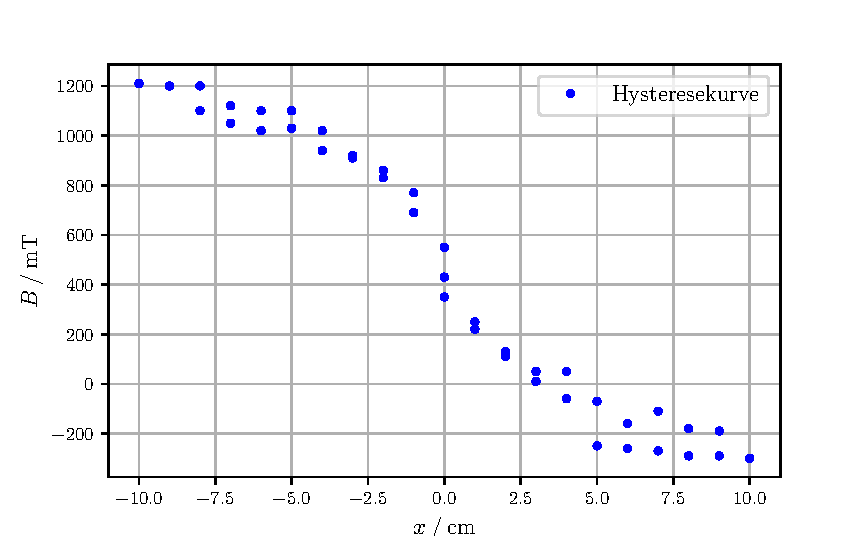
\includegraphics[width=\textwidth]{build/Hysteresekurve.pdf}
  \caption{Messdaten der Ringspule zu einer Hysteresekurve aufgetragen.}\label{fig:hysterese}
\end{figure}

Anhand der Messdaten der Tabelle wird die Koerzitivfeldstärke, die Remanenz
und Sättigungsmagnetisierung bestimmt.
Die Remanenz kann dabei direkt der Tabelle entnommen werden. Sie nimmt je nach dem, welcher Weg 
auf der Hysteresekurve genommen wird, zwei verschiedene Werte an.

\quad $B_{R}^1=430 \si{\milli\tesla}$ 
\quad $B_{R}^2=550 \si{\milli\tesla}$

Um die Hysteresekurve zu erstellen muss vorerst die magnetische Feldstärke im inneren der Ringspule berechnet werden.
Zum Berechnen der Feldstärke im inneren einer Ringspule kann die Gleichung 

\begin{equation}
H=\frac{NI}{2\pi R}
\end{equation}

verwendet werden. Hierbei entspricht $N$ die Anzahl der Windungen, I ist der anliegende Strom und 
R entspricht dem Radius des Torus. Da es sich aber ledeglich um eine fast geschlossene Ringspule handelt, muss die Breite des Luftspaltes
noch von der Länge der Spule abgezogen werden. Damit ergibt sich die Gleichung:

\begin{equation}
H=\frac{NI}{2\pi R-d_l}
\end{equation}

Da laut Konvention der Strom beim entlang gehen der Neukurve im Uhrzeigersinn fließen soll, aber 
bei der Versuchsdurchführung links laufendem Strom begonnen worden ist, wird die Ausrichtung der Hysteresekurve
durch das Hinzufügen eines negativen Vorzeichens der Konvention angepasst. Dabei wird das experiementelle
Ergebnis nicht verändert.
Nach einfügen aller bekannter Werte kann $H$ als Funktion von $I$ bestimmt werden:

\begin{equation}
H(I)=-\frac{595\cdot I}{2\pi \cdot 0.185\si{\m}-0.003\si{\m}}
\end{equation}

Die Koerzitivfeldstärke wird auf Grund der wenigen Messdaten durch eine Ausgleichsgerade bestimmt, dessen
Nulldurchgang in guter Näherung der Koerzitivfeldstärke entspicht.

\begin{equation}
g_i(H)=m_i\cdot H+b_i
\end{equation}
  
Dabei berechnen sich die $m_i$ und $b_i$ wie folgt:

\begin{gather}
m_1=\frac{H(4)-H(3)}{-60-10} \\
m_2=\frac{H(4)-H(5)}{50-(-250)}\\
b_1=10-m_1\cdot H(3)\\
b_2=50-m_2\cdot H(4)
\end{gather}

Um die Koerzitivfeldstärken zu erhalten, muss die Nullstelle der beiden Geraden berechnet werden. \quad $g_i(H) \stackrel{!}{=}0$\\
Das nach $H$ umgeformt ergibt:

\begin{equation}
H_{i}^{c}=\frac{-b_i}{m_i}
\end{equation}

Nach Einsetzen aller Werte folgt für die Koerzitivfeldstärken:

\quad $H_{1}^{c}\cong -1612.9181 \frac{\si{\ampere}}{\si{\m}}$
\quad $H_{2}^{c}\cong -2138.3384 \frac{\si{\ampere}}{\si{\m}}$

Die Sättigungsmagnetisierung lässt sich näherungsweise aus der Tabelle ablesen, da bei betragsmäßig hohen
Strömen sich der magnetische Fluss kaum noch ändert. So ergeben sich zwei Werte für die Sättigungsmagnetisierung:

\quad $B_{1}^{s}\cong -300 \si{\milli\tesla}$
\quad $B_{2}^{s}\cong 1210 \si{\milli\tesla}$























